% !TeX root = ../../tesis.tex

% =============================================================================
\subsection*{Grupo 1: Indicadores Espaciales y de Cobertura}
% =============================================================================

% -----------------------------------------------------------------------
\subsection{Nivel de Cobertura de la Red de Transporte \texorpdfstring{$C$}{C}}
\label{subsec:indicador-cobertura}
% -----------------------------------------------------------------------

\textbf{Fuente principal:} \citet{fortin2016innovative}

\subsubsection{Definición y Fundamentación}

El nivel de cobertura es el indicador de entrada del modelo: el más
independiente de todos, pues su cálculo se realiza exclusivamente mediante
análisis espacial y no requiere que el grafo de la red esté completamente
interconectado. Mide la proporción del territorio urbano que queda dentro de una
distancia caminable de algún nodo de la red de transporte.

\citet{fortin2016innovative} explican en su sección de evaluación de
accesibilidad que los indicadores de cobertura más comunes se calculan trazando
áreas de influencia ---típicamente un \textit{buffer} de 500 metros o 400 metros
como radio de caminata promedio aceptable--- alrededor de cada parada de la red.
A partir de estas áreas, es posible identificar la proporción de individuos o de
empleos que quedan dentro de cierta distancia de la infraestructura de
transporte, lo que permite evaluar el nivel de accesibilidad en el territorio y
señalar con precisión los lugares donde deben ocurrir las mejoras.

\subsubsection{Fórmula}

\begin{equation}
    C = \frac{\text{Área Cubierta por Buffers}}{\text{Área Total de la Zona de Estudio}}
    \label{eq:cobertura}
\end{equation}

Donde:
\begin{itemize}
    \item $C$ = Nivel de Cobertura de la Red (adimensional, rango $[0, 1]$).
\item \textbf{Área Cubierta} = Unión de los polígonos de cobertura (isócronas o
    \textit{buffers} circulares) generados alrededor de cada parada de la red,
    medida en km².
\item \textbf{Área Total} = Superficie del polígono urbano delimitado de la zona
    de estudio, en km².
\end{itemize}

\begin{figure}[H]
    \centering
    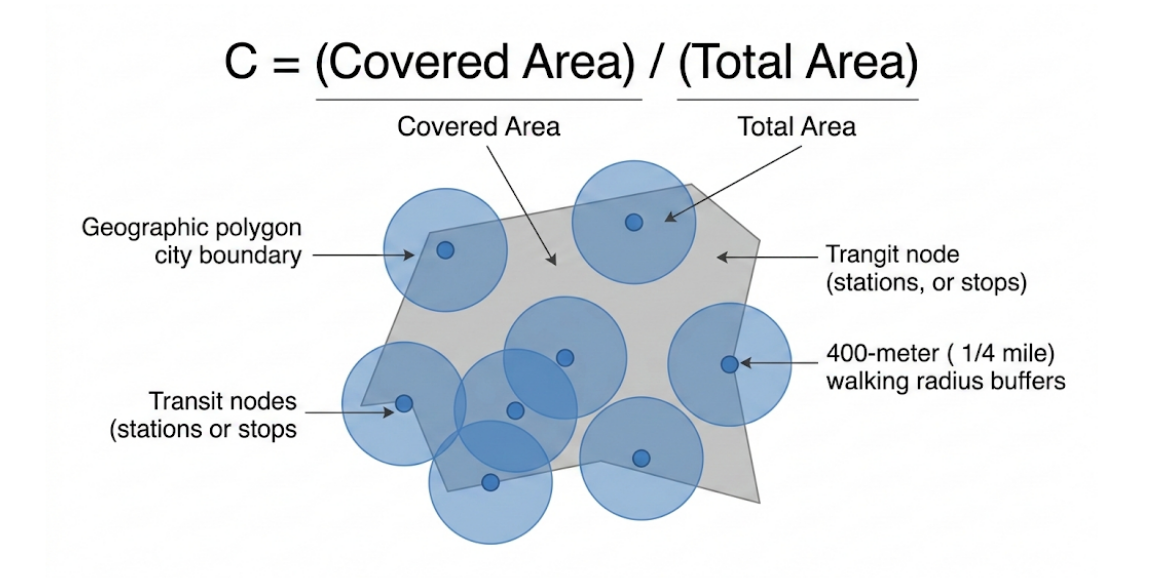
\includegraphics[width=0.80\textwidth]{Figures/Cap3/CoberturaTransporte.png}
    \caption[Diagrama del indicador de Cobertura $C$]{Esquema del cálculo del
indicador $C$: polígono de la zona de estudio (Área Total), nodos de transporte
    y círculos de radio 400\,m (Área Cubierta).}
    \label{fig:indicador-C}
    \fuentefigura{Elaboración propia con base en \citet{fortin2016innovative}.}
\end{figure}


\subsubsection{Consideraciones de Implementación}

Para una representación más precisa que la del \textit{buffer} circular
estático, se implementará el concepto de \termino{isócronas}: áreas de
influencia construidas a partir de la red vial real de OpenStreetMap, que
delimitan todos los puntos alcanzables caminando desde una parada en exactamente
15 minutos a la velocidad promedio peatonal (4.5 km/h en zonas densas). Las
isócronas producen polígonos irregulares que respetan barreras físicas como vías
rápidas, cuerpos de agua o pendientes pronunciadas, ofreciendo una medida de
cobertura sustancialmente más realista que un círculo uniforme.

El resultado de las isócronas se superpone al censo poblacional del INEGI para
calcular no solo el área cubierta, sino la \termino{población cubierta}: la
fracción de habitantes de la zona metropolitana que reside dentro del área de
influencia de alguna parada de la red.

\subsubsection{Ejemplo Práctico: \cdmx{} y Zona Metropolitana}

\textbf{Datos de entrada:} Coordenadas georreferenciadas de todas las paradas de
la red (Metro, Metrobús, RTP, Trolebús, Cablebús, Mexibús) en formato
\geojson{} ; polígono del área urbana de la \zmvm{} $\approx 7{,}866$\,km²; capa
de manzanas del INEGI con datos de población del Censo 2020.


\begin{table}[H]
    \centering
    \caption{Estimaciones del indicador $C$ por escenario de red.}
    \label{tab:cobertura-escenarios}
    \begin{tabularx}{\textwidth}{X r r}
        \toprule
        \textbf{Escenario} & \textbf{Área Cubierta} & \textbf{Cobertura $C$} \\
        \midrule
        Red masiva actual (solo Metro + Metrobús + Cablebús)
            & $\approx 450$\,km² & $C \approx 0.06$ \\
        Red completa actual (incluyendo RTP y concesionados)
            & $\approx 2{,}800$\,km² & $C \approx 0.36$ \\
        Red con propuesta del Anillo Periférico (+60 estaciones)
            & $\approx 3{,}150$\,km² & $C \approx 0.40$ \\
        \bottomrule
    \end{tabularx}
\end{table}

La implementación computacional de referencia para este indicador se encuentra
en el \autoref{anx:indicadores-implementacion} (§\ref{anx:impl-cobertura}).

Este indicador da cumplimiento al Objetivo Específico 4 (§
\ref{subsec:obj-especificos}): la cobertura $C$ medida por cuadrante geográfico
y por sistema es la métrica primaria para delimitar las zonas periféricas con
mayor déficit de acceso estructurado, que son el punto de partida para evaluar
la pertinencia del escenario hipotético anillar.
